\cotefile{74}
\scanpage{106}
\figure{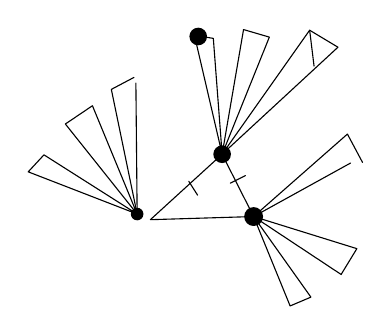
\begin{tikzpicture}[x=0.008cm,y=-0.008cm,line cap=round,line join=round]
\draw (237,514)--(351,410)--(401,509)--cycle;
\draw (216,505)--(43,438)--(68,411)--cycle;
\draw (216,505)--(102,362)--(145,333)--cycle;
\draw (216,505)--(175,307)--(211,288);
\draw (216,505)--(214,297);
\draw (351,410)--(307,221)--(337,226)--cycle;
\draw (351,410)--(385,212)--(426,224)--cycle;
\draw (351,410)--(490,213)--(535,240)--cycle;
\draw (490,213)--(497,270);
\draw (401,509)--(550,378)--(574,423);
\draw (401,509)--(555,424);
\draw (401,509)--(565,560)--(540,601)--cycle;
\draw (401,509)--(492,637)--(459,651)--cycle;
\draw (298,453)--(312,475);
\draw (364,456)--(388,444);
\fill (216,505) circle[radius=10];
\fill (351,410) circle[radius=14];
\fill (401,509) circle[radius=15];
\fill (313,223) circle[radius=14];

\end{tikzpicture}}

$\sigma_{t_0}$

\figure{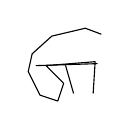
\begin{tikzpicture}[x=0.025cm,y=-0.025cm,line cap=round,line join=round]
\draw (39,4)--(31,1)--(14,5)--(4,14)--(2,23)--(8,35)--(17,38)--(20,29)--(11,20)--(36,18)--(35,34);
\draw (6,20)--(37,19);
\draw (21,20)--(25,34);


\end{tikzpicture}}

\figure{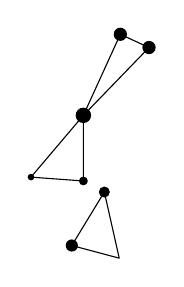
\begin{tikzpicture}[x=0.007cm,y=-0.007cm,line cap=round,line join=round]
\draw (1123,378)--(1218,266)--(1218,385)--cycle;
\draw (1218,266)--(1285,119)--(1337,143)--cycle;
\draw (1197,502)--(1256,405)--(1283,525)--cycle;
\fill (1218,266) circle[radius=14];
\fill (1285,119) circle[radius=12];
\fill (1337,143) circle[radius=12];
\fill (1123,378) circle[radius=6];
\fill (1218,385) circle[radius=8];
\fill (1197,502) circle[radius=11];
\fill (1256,405) circle[radius=10];

\end{tikzpicture}}

\figure{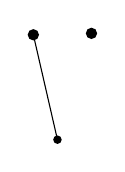
\begin{tikzpicture}[x=0.009cm,y=-0.009cm,line cap=round,line join=round]
\draw (209,699)--(243,847);
\fill (209,699) circle[radius=8];
\fill (243,847) circle[radius=6];
\fill (291,697) circle[radius=8];

\end{tikzpicture}}

\textcircled{\unsure{bons|bon}} \uline{\unsure{compl.} : $0$ \unsure{branches|boucles}} \quad a)

\figure{
\begin{tikzpicture}[x=0.035cm,y=-0.035cm,line cap=round,line join=round]

\fill (0,8) circle[radius=8];
\fill (31,5) circle[radius=5];
\fill (56,0) circle[radius=4];

\end{tikzpicture}}

par un sommet passe $0$ triangle (\deleted{\illegible{1}} : $0$ arêtes)

\noindent\rule{.69\linewidth}{.4pt}

\textcircled{\uline{\unsure{bons|bon}}} \quad $n=1$ branche \quad b)

\figure{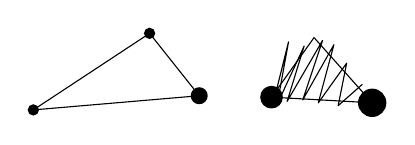
\begin{tikzpicture}[x=0.018cm,y=-0.018cm,line cap=round,line join=round]
\draw (0,54)--(82,0)--(117,44)--cycle;
\draw (168,45)--(198,3)--(239,49)--cycle;
\draw (170,46)--(180,6)--(172,50)--(191,9)--(179,48)--(204,5)--(190,47)--(212,8)--(201,49)--(221,21)--(215,51)--(232,36);
\fill (0,54) circle[radius=4];
\fill (82,0) circle[radius=4];
\fill (117,44) circle[radius=6];
\fill (168,45) circle[radius=8];
\fill (239,49) circle[radius=10];

\end{tikzpicture}}

par un sommet passe $1$ triangle exact\textsuperscript{t} (ou $2$ arêtes exact\textsuperscript{t})

\noindent\rule{.81\linewidth}{.4pt}

% slanted
\margin{cas où existe un centre (un pt auquel tt autre pt est lié) -- (unique sauf pour le cas où $S$ est \unsure{bon|borné} $=$ un triangle)}

\uline{non bons} \qquad c)

\figure{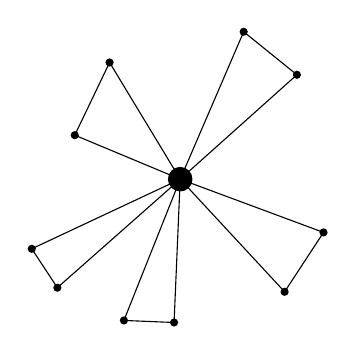
\begin{tikzpicture}[x=0.013cm,y=-0.013cm,line cap=round,line join=round]
\draw (1020,1032)--(917,989)--(951,918)--cycle;
\draw (1020,1032)--(1082,888)--(1134,930)--cycle;
\draw (1020,1032)--(1160,1084)--(1122,1142)--cycle;
\draw (1020,1032)--(1014,1172)--(965,1170)--cycle;
\draw (1020,1032)--(900,1138)--(875,1100)--cycle;
\fill (1020,1032) circle[radius=12];
\fill (917,989) circle[radius=4];
\fill (951,918) circle[radius=4];
\fill (1082,888) circle[radius=4];
\fill (1134,930) circle[radius=4];
\fill (1160,1084) circle[radius=4];
\fill (1122,1142) circle[radius=4];
\fill (1014,1172) circle[radius=4];
\fill (965,1170) circle[radius=4];
\fill (900,1138) circle[radius=4];
\fill (875,1100) circle[radius=4];

\end{tikzpicture}}

\[ n\geq 2\ \text{branches} \]

\deleted{\unsure{type}} étoile de triangles \deleted{\unsure{telle que}} \deleted{\unsure{en des sommets|à deux sommets}} tous les sommets sauf $1$ sont d'ordre $2$, \deleted{l'autre} (l'\unsure{exceptionnel|exceptionn\textsuperscript{el}} est d'ordre $\geq4$)

par tous les sommets sauf $1$ passe exact\textsuperscript{t} un triangle, pour l'excep. il y en a \deleted{\unsure{au}} au moins deux [\deleted{\unsure{et}} \unsure{i.e.|i.e} il y a au moins $4$ de sommets par lesquels passe \deleted{\unsure{un}} exact\textsuperscript{t} $1$ triangle ..]

\noindent\rule{\linewidth}{.4pt}

\uline{bons}, Par tt sommet passe au moins $\unsure{3|2}$ triangles

% archive sheet number: 105
\scanpage{107}
\uline{Automorphismes des \deleted{complexes} \inserted{graphes} trialitaires}.

Soit $(S,A)$ un \deleted{complexe} \inserted{graphe} trialitaire, $\underline t=\{a,b,c\}$ un triangle. On a défini une bijection involution \deleted{$\unsure{\sigma_t|\sigma_{\underline t}}$ de $\unsure{S|S,S}$}

\[ \sigma_{\underline t}=\sigma_{\{a,b,c\}}: S\mathrel{\unsure{-|\to}}S \]

par

\[
\begin{aligned}
\sigma_{\underline t}\mid\underline t&=\mathrm{id}_{\underline t}\\
\sigma_{\underline t}\mid E_a^{\unsure{t|\underline t}}\deleted{\unsure{(t)}}&=\sigma_a^{\underline t}
\qquad\text{(transforme $x\in E_a$ en l'unique}\\[-2pt]
&\hspace{7em}\text{él de $E_a$ lié à $x$)}
\end{aligned}
\]

\uline{Proposition} \qquad a) $\sigma_{\underline t}$ est un automorphisme du \deleted{complexe} graphe $(S,A)$, et $\underline t$ est l'ens des pts fixes de $\sigma_{\underline t}$.

b) L'application $\underline t\longmapsto\sigma_{\underline t}$ de $T$ dans $G=\mathrm{Aut}(S,A)$ est injective, et a comme image l'ens des autom involutifs \inserted{$u$} de $(S,A)$ tels que \deleted{l'ens des} $\operatorname{card} S^u=3$

C'est $\pm$ évident\ldots

Soit $G\unsure{=|\neq}\mathrm{Aut}(S,A)$. Les $\sigma_t$ sont $\in G$. Soit $G^{\unsure{0|\circ}}$ le grpe qu'ils engendrent. Si $g\in G$, on a

\[ \operatorname{int}(g).\sigma_t=g\,\sigma_t\,g^{-1}=\sigma_{g(t)} \]

donc $G^0$ est un ss. grpe invariant.

% archive sheet number: 106
\scanpage{108}
\uline{Théorème} $G^{\unsure{0|\circ}}$ est transitif sur l'ens des arcs de $(S,A)$ (\unsure{lire|i.e.} des couples $(s,t)$ de deux pts liés) et a fortiori sur l'ens des sommets, \deleted{et} \inserted{l'ens des arêtes et} sur l'ens des triangles (\inserted{ensemble} qui sont isom. à des ens. quotients de l'ens précédent.)

% slanted
\margin{Sauf exception $c\,(=\operatorname{Card} E_a)=1$ i.e. $(S,A)$ est le bi-triangle. Alors $G$ a les transitivités \unsure{énoncées} pour $G^0\inserted{\unsure{\simeq}\mathfrak S_3\times\mathfrak S_3}$, qui est d'indice $2$ dans $G$ (\deleted{\unsure{Aut}} $\mathfrak S_2.(\mathfrak S_3\times\mathfrak S_3)$). $G^0$ est encore transitif sur $S$, mais pas sur $\deleted{\unsure{A}}T$ (ni à fortiori sur $A$) -- il est transitif sur chacune des deux familles de triangles parallèles\ldots}

\uline{Cor} Les $\sigma_{\underline t}$ $(\underline t\in T)$ sont conjugués \inserted{dans $G^0$ (a fortiori en $G$)}, et forment exactement une classe de conjugaison d'éléments de $G^0$ (ou de $G$)

Résulte des deux lemmes suivants

\uline{Lemme 1} Soient $s,t\in S$, alors

a) Si $s,t$ sont liés, $\exists\ \underline t\in T$ tel que $t=\sigma_{\underline t}s$

b) \deleted{Si $s,t$ sont non liés} \inserted{Dans tous les cas} $\exists\ u\in S$ tel que $s$ lié à $u$ et $u$ lié à $t$, donc (vu a) des $\underline t,\underline t'\in T$ tels que $u=\sigma_{\underline t}s$, $t=\sigma_{\underline t'}u$, donc $t=\sigma_{\underline t'}\sigma_{\underline t}s$.

Le lemme a) est clair (\deleted{prendre pour $\underline t$} \inserted{soit $a$ le troisième sommet du triangle défini par $\{s,t\}$}, \deleted{le triangle défini \unsure{ces trois|un triangle}} et soit $\underline t$ \unsure{un} triangle de sommet $a$ distinct du précédent) ; d'où immédiatement b.

\uline{Lemme 2} \inserted{(\unsure{Supposons|Supposant} $c\neq1$, i.e. il y a au moins $3$ triangles incidents en chaque sommet\ldots} Soient $a\in S$ et $s,t$ deux él. de $S$ liés à $a$, \inserted{$\unsure{s\neq t}$ et $s$ non lié à $t$.} Alors $\exists\,g\in G^0$ (produit \deleted{de deux} $\sigma_{\unsure{\underline\tau|\underline t}} \sigma_{\underline t}$, où $\underline\tau,\underline t$ sont $2$ triangles distincts convenables) tels que $u(a)=a$, $u(s)=t$, $u(t)=s$

% archive sheet number: 107
\scanpage{109}
Plus précisément, si $\underline t_0\inserted{=\{a,b,c\}}$ est un triangle de sommet $a$ ne contenant ni $s$ ni $t$ (il y en a par l'hyp. que $c\neq1$ i.e. $c\geq2$), on peut choisir de plus $u$ (i.e. $\underline t,\unsure{\underline t'|\underline\tau}$) tel que \deleted{$ua=a,\ ub=c,\ uc=b$} \inserted{$u\mid\underline t_0=\mathrm{id}_{\underline t_0}$ (i.e., $ua=a,\ ub=b,\ uc=c$} \deleted{\unsure{$b,c$} et $ua=a,\ ub=c,\ uc=b$.}

\figure{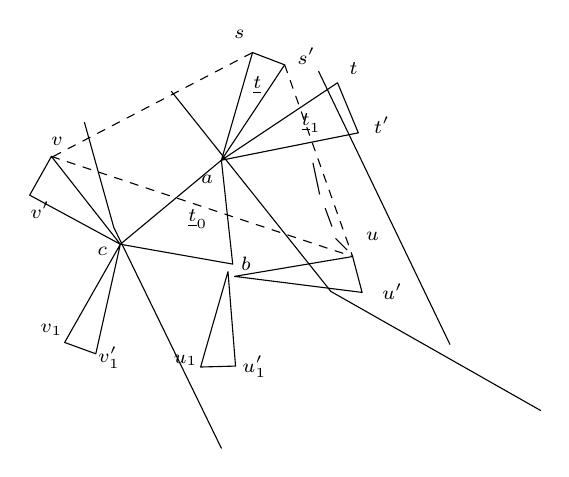
\begin{tikzpicture}[x=0.012cm,y=-0.012cm,line cap=round,line join=round]
\draw (233,394)--(126,483)--(245,504)--cycle;
\draw (233,394)--(266,280)--(300,293)--cycle;
\draw (233,394)--(356,312)--(378,365)--cycle;
\draw (126,483)--(53,390)--(30,431)--cycle;
\draw (126,483)--(67,587)--(100,599)--cycle;
\draw (240,512)--(211,613)--(248,612)--cycle;
\draw (247,517)--(372,496)--(382,534)--cycle;
\draw (330,397)--(337,430);
\draw (343,445)--(350,464);
\draw (354,477)--(366,489);
\draw (88,354)--(119,465)--(233,699);
\draw (180,321)--(349,533)--(571,659);
\draw (336,300)--(475,589);

\node[inner sep=1pt,font=\scriptsize] at (218,414) {$a$};
\node[inner sep=1pt,font=\scriptsize] at (259,504) {$b$};
\node[inner sep=1pt,font=\scriptsize] at (107,490) {$c$};
\node[inner sep=1pt,font=\scriptsize] at (208,456) {$\underline t_0$};
\node[inner sep=1pt,font=\scriptsize] at (252,261) {$s$};
\node[inner sep=1pt,font=\scriptsize] at (323,284) {$s'$};
\node[inner sep=1pt,font=\scriptsize] at (271,315) {$\underline t$};
\node[inner sep=1pt,font=\scriptsize] at (373,297) {$t$};
\node[inner sep=1pt,font=\scriptsize] at (403,357) {$t'$};
\node[inner sep=1pt,font=\scriptsize] at (328,355) {$\underline t_1$};
\node[inner sep=1pt,font=\scriptsize] at (59,374) {$v$};
\node[inner sep=1pt,font=\scriptsize] at (41,447) {$v'$};
\node[inner sep=1pt,font=\scriptsize] at (393,475) {$u$};
\node[inner sep=1pt,font=\scriptsize] at (414,533) {$u'$};
\node[inner sep=1pt,font=\scriptsize] at (53,574) {$v_1$};
\node[inner sep=1pt,font=\scriptsize] at (114,603) {$v'_1$};
\node[inner sep=1pt,font=\scriptsize] at (195,606) {$u_1$};
\node[inner sep=1pt,font=\scriptsize] at (268,613) {$u'_1$};
\draw[dashed] (55,390)--(266,280);
\draw[dashed] (300,293)--(372,496);
\draw[dashed] (53,390)--(372,496);
\end{tikzpicture}}

\deleted{\unsure{Théor.} \unsure{Variante|Nouveau} On peut trouver $v\in G^0$ tel que $v\mid\underline t_0=\underline t_0$ ($va=a,vb=b,vc=c$) et $vs=t$}

\deleted{\uline{\unsure{Récette|Recette}} On \deleted{choisit $u$ lié à $t$ et $s$} complète les triangles $\underline t=\{a,s,s'\}$ et $\underline t_0=\{a,b,c\}$ (par $s'$ et $c$). \unsure{On} \deleted{\unsure{pour} $\unsure{\underline t=} $} a donc $\widetilde{\underline E}_a,\widetilde E_b,\widetilde{\underline E}_c$ etc \ldots) on choisit \textcircled{$u$} \inserted{$\neq a$} lié à $b$ et à $s$ i.e. $u\in\widetilde E_b$ lié à $s$, on complète en triangle $\{s,u,v\}$ sur $(a,b,c)$, donc}

\figure{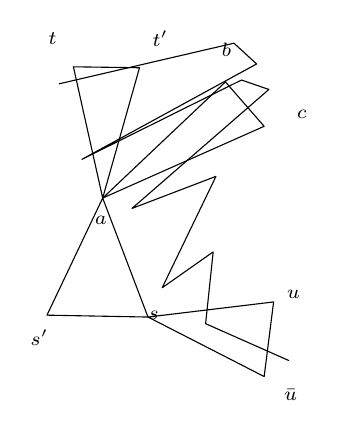
\begin{tikzpicture}[x=0.012cm,y=-0.012cm,line cap=round,line join=round]
\draw (156,1044)--(125,905)--(195,906)--cycle;
\draw (156,1044)--(286,921)--(327,968)--cycle;
\draw (156,1044)--(97,1168)--(204,1170)--cycle;
\draw (204,1170)--(337,1154)--(327,1233)--cycle;
\draw (110,923)--(295,880)--(319,902)--(134,1003)--(303,919)--(332,929)--(187,1055)--(276,1021)--(219,1139)--(273,1101)--(265,1177)--(353,1216);

\node[inner sep=1pt,font=\scriptsize] at (103,875) {$t$};
\node[inner sep=1pt,font=\scriptsize] at (217,875) {$t'$};
\node[inner sep=1pt,font=\scriptsize] at (287,887) {$b$};
\node[inner sep=1pt,font=\scriptsize] at (367,955) {$c$};
\node[inner sep=1pt,font=\scriptsize] at (154,1068) {$a$};
\node[inner sep=1pt,font=\scriptsize] at (89,1192) {$s'$};
\node[inner sep=1pt,font=\scriptsize] at (210,1168) {$\unsure{s}$};
\node[inner sep=1pt,font=\scriptsize] at (358,1146) {$u$};
\node[inner sep=1pt,font=\scriptsize] at (355,1252) {$\bar u$};
\end{tikzpicture}}

\[
\deleted{\begin{aligned}
u\in\widetilde E_b,\ v\in\widetilde E_c &\qquad \{s,u,v\}\in\widetilde T\subset T\\
u'\in\widetilde E_b,\ v'\in\widetilde E_c &\qquad (s',u',v')\in\widetilde T\subset T
\end{aligned}}
\]

\deleted{d'où}

\[ \deleted{\left[\begin{aligned}(b,u,u')&\in T\\(c,v,v')&\in T\end{aligned}\right]} \]

\deleted{\deleted{On \unsure{prend|peut} choisit} Quitte à échanger $t,t'$ \unsure{O.P.S} $t$ lié à $u$, \deleted{\unsure{$t=$}} complétons alors en le triangle}

\[ \deleted{(t,u,\underset{\substack{\unsure{\rotatebox{-90}{$\in$}|\uparrow}\\ \widetilde E_c}}{v_1})\in\widetilde T} \]

\deleted{Alors $t'$ est lié à $u'$, donc pas à $v'$, donc à $v$ et complétons $(t',v)$ en triangle}

\[ \deleted{(t',v,\underset{\substack{\unsure{\rotatebox{-90}{$\in$}|\uparrow}\\ \widetilde E_b}}{u_1})\in\widetilde T\subset T} \]

\deleted{Et avec $u_1,v_1$ on a aussi}

\[ \deleted{u'_1\in\widetilde E_b,\quad v'_1\in\widetilde E_c\qquad \{b,u_1,u'_1\},\ \{c,v_1,v'_1\}\in T} \]

% archive sheet number: 108
\scanpage{110}
\deleted{Ceci posé, on prendra}

\[ \deleted{\tau=\{t',u',v'_1\},\quad \tau'=\{t',u_1,\unsure{v|w|v_1}\}} \]

\begin{center}---\end{center}
Changeons de notation donnés $a,s,t$ ($s,t$ liés à $a$, distincts et non liés) on complète triangles (distincts) $\{a,s,s'\}$, $\{a,t,t'\}$, on a triangle $\underline t_0$ de sommet $a$ distinct des $2$ précédents

% slanted
\margin{(Pour l'existence, \unsure{rapporter} la situation au triangle de base $\{a,s,s'\}$ -- il y a exactement \uline{$c$} choix \unsure{pour|de} $u$}

\figure{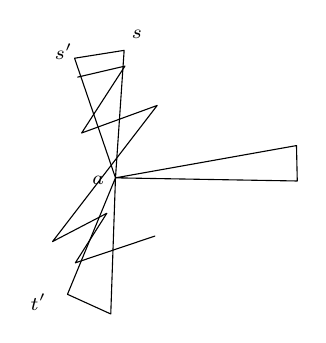
\begin{tikzpicture}[x=0.01cm,y=-0.01cm,line cap=round,line join=round]
\draw (263,757)--(211,605)--(274,595)--cycle;
\draw (263,757)--(493,716)--(494,761)--cycle;
\draw (263,757)--(202,905)--(257,930)--cycle;
\draw (215,629)--(275,615)--(220,700)--(316,665)--(183,838)--(252,802)--(212,865)--(313,831);

\node[inner sep=1pt,font=\scriptsize] at (197,597) {$s'$};
\node[inner sep=1pt,font=\scriptsize] at (290,575) {$s$};
\node[inner sep=1pt,font=\scriptsize] at (241,760) {$a$};
\node[inner sep=1pt,font=\scriptsize] at (165,915) {$t'$};
\end{tikzpicture}}

On choisit $u\neq a$ lié à $s$ et à $t$ (il est lié à un unique sommet de $\underline t_0$, qui est distinct de $a$, soit $b$), on prend $\{s,u,v\}\in T$, $\{t,u,w\}\in T$, \deleted{ils} \inserted{$v,w$} sont liés à $c$ (et sont distincts de $a,b$), on prend les triangles $\underline\sigma=\{c,v,v'\}$ et $\underline\tau=\{c,w,w'\}$, et on considère les symétries $\sigma_{\underline\sigma},\sigma_{\underline\tau}$, qui commutent (car $\underline\sigma,\underline\tau$ sont des triangles sécants).

\figure{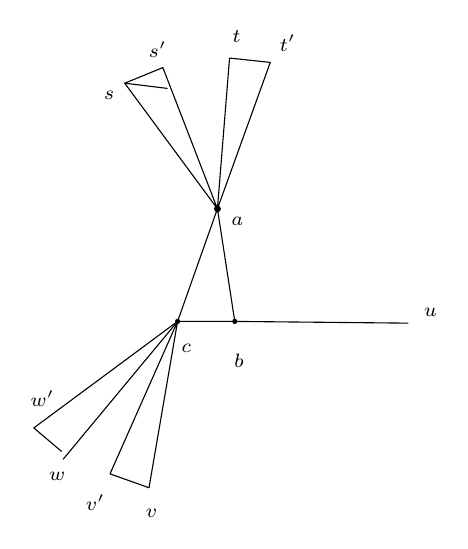
\begin{tikzpicture}[x=0.011cm,y=-0.011cm,line cap=round,line join=round]
\draw (237,1158)--(130,1013)--(174,995)--cycle;
\draw (130,1013)--(179,1019);
\draw (237,1158)--(251,984)--(298,989)--cycle;
\draw (237,1158)--(191,1288)--(257,1288)--cycle;
\draw (257,1288)--(457,1290);
\draw (191,1288)--(25,1411)--(57,1438);
\draw (191,1288)--(59,1447);
\draw (191,1288)--(113,1464)--(158,1480)--cycle;
\fill (237,1158) circle[radius=4];
\fill (191,1288) circle[radius=3];
\fill (257,1288) circle[radius=3];
\node[inner sep=1pt,font=\scriptsize] at (112,1027) {$s$};
\node[inner sep=1pt,font=\scriptsize] at (168,974) {$s'$};
\node[inner sep=1pt,font=\scriptsize] at (259,959) {$t$};
\node[inner sep=1pt,font=\scriptsize] at (318,967) {$t'$};
\node[inner sep=1pt,font=\scriptsize] at (260,1173) {$a$};
\node[inner sep=1pt,font=\scriptsize] at (201,1319) {$c$};
\node[inner sep=1pt,font=\scriptsize] at (262,1334) {$b$};
\node[inner sep=1pt,font=\scriptsize] at (483,1277) {$u$};
\node[inner sep=1pt,font=\scriptsize] at (35,1377) {$w'$};
\node[inner sep=1pt,font=\scriptsize] at (52,1467) {$w$};
\node[inner sep=1pt,font=\scriptsize] at (96,1497) {$v'$};
\node[inner sep=1pt,font=\scriptsize] at (161,1510) {$v$};
\end{tikzpicture}}

On a

\[
\begin{aligned}
\sigma_{\underline\sigma}s&=u &\text{car }\{s,u,v\}&\in T,\ v\in\underline\sigma\\
\sigma_{\underline\tau}u&=t &\text{car }\{t,u,w\}&\in T,\ w\in\unsure{\underline T|\underline\tau}
\end{aligned}
\]

% slanted
\margin{\deleted{\uline{NB} $\sigma_{\underline\sigma}u=s$ \quad $\sigma_{\underline\tau}s=u$ donc \deleted{\unsure{$s\leftrightarrow u$}} $Uu=\mathrm{id}$, \deleted{donc} \unsure{$U$ transforme|et transforme} $\{s,u,v\}\in\widetilde T$ en $\{t,u,w\}\in\widetilde T$}}

enfin, $\sigma_{\underline\sigma}$ et $\sigma_{\underline\tau}$ échangent $a$ et $b$ \inserted{et fixent $c$}, donc leur produit fixe les pts $a,b,c$. Donc $U=\sigma_{\underline\sigma}\,\sigma_{\underline\tau}$ transforme $(a,s)$ en $(a,t)$ et induit l'identité \deleted{sur} $(a,b,c)$

\deleted{\uline{NB} Supposons qu'on ait $r\in\widetilde E_c$ lié à $s$ et à $t$. Comme $s$ lié à $v$ (\deleted{\unsure{et|donc}} non à $v'$) $t$ lié à $w$ (donc non à $w'$), on a $r\neq v',w'$}

% archive sheet number: 109
\scanpage{111}
\uline{Corollaire} Considérons le sous grpe \inserted{(invariant) $H^{\unsure{0|\circ}}$} du grpe \deleted{$\unsure{G}$} \inserted{$H={}$}$\underline{\mathrm{Aut}}(S,A\,;a,b,c)$ \deleted{engendré} \inserted{formé} par les produits d'un nb pair de symétries $\sigma_{\underline t}$ relatifs à des triangles verticaux.

Alors $H^0$ est transitif sur l'ens $\widetilde T$ des triangles supérieurs. De façon précise, si $\deleted{\unsure{\underline s,\underline t'}}\inserted{\underline s,\underline t}\in\widetilde T$, et si $a\in\underline t_0$, soit \deleted{$u\in$} $b\in t_0$, $b\neq a$ tel que $\exists\,u\in\widetilde E_b$ lié aux deux sommets \inserted{$s,t$} de $\underline s\ \underline t$ sur $a$, alors $\exists$

\deleted{produit $U$ de deux symétries \deleted{relatifs} $\sigma_{\unsure{v}},\sigma_{w}$ ($v,w\in E_c=\widetilde E_c/2$) tel que $Us=t$, \inserted{$U\underline s$ et $\underline t$ coïncident \uline{en $a$} ;} et on a ensuite \uline{le choix} pour trouver $V$, produit de deux symétries \unsure{latérales|relatives} en $b$, ou en $c$, tels que $VU\underline s=\underline t$.}

\deleted{Si on le prend en $\underline c$, comme $V$ et $U$ commutent, $VU$ sera encore un autom. involutif}

% archive sheet number: 110
\scanpage{112}
\uline{Lemme 1} \inserted{(cas $\unsure{c|S}$ fini $\neq1,2$)} Soient $s,t\in\widetilde E_a$, alors $\exists\,s_1\in\widetilde E_a$, et $u,v\in\widetilde E_b$ tels que $u$ soit lié à $s$ et $s_1$, $v$ lié à $s_1$ et $t$.

% slanted
\margin{C'est \uline{faux} si $c=1,2$}

Soit $\widetilde E_{b}(s)=\{u\in\widetilde E_b\mid u\text{ lié à }s\}$, de $=$ $\widetilde E_b(t)$, ils sont de cardinal $c$ (des sections de $\widetilde E_b$ sur $E_b$) Si $\widetilde E_b(s)\cap\widetilde E_b(t)\neq\emptyset$, il suffit de prendre $u=v$ \deleted{\unsure{dans|élt}} dans cette intersection et $\bar s_1=s$. Sinon, comme $\operatorname{Card}\widetilde E_b=2c$, on a

\[ \widetilde E_b\deleted{\unsure{\varnothing}}=\underset{\substack{\shortparallel\\ B'}}{\widetilde E_b(s)}\amalg\underset{\substack{\shortparallel\\ B''}}{\widetilde E_b(t)} \]

(\unsure{ou mm|ou non|ou même|comme même} $\widetilde E_b(t)=\widetilde E_b(s')$ et sans doute cela impliquera $t=s'$, mais pour l'instant on ne peut le prouver). On cherche \deleted{\unsure{donc}} $\bar s_1$ tel que $\widetilde E_b(\bar s_1)\cap\widetilde E_b(s)\neq\emptyset$, $E_b(\bar s_1)\cap\widetilde E_b(t)\neq\emptyset$.

Si un tel $\bar s$ n'existait pas, on aurait $\forall\,\unsure{r|\bar r}\in\widetilde E_a,\ \widetilde E_b(\unsure{r|\bar r})$ est contenu dans \deleted{$\widetilde E_b(s)$} $B'$ ou $B''$ et pour des raisons de cardinal (comme il est lui $=$ de cardinal $c$) on aurait

\[ \forall r\in A=\widetilde E_a,\qquad \text{on a}\quad \widetilde E_b(r)=B'\ \text{ou}\ \widetilde E_b(r)=B'' \]

Soit

\[
\begin{aligned}
A'&=\{r\in A\mid\widetilde E_b(r)=B'\},& A''&=\{r\in A\mid\widetilde E_b(r)=B''\}\\
&&&=\complement_AA'
\end{aligned}
\]

donc \deleted{$A'=\sigma_{\underline t_0}A'',\ A''=\sigma_b A'$, et \unsure{pour}} $\forall$ couple $r,r'$ de pts de $A$ liés, un et un seul de $r,r'$ est dans $A'$, l'autre dans $A''$ -- donc $A',A''$ sont des sections complémentaires de $\widetilde E_a$ sur $E_a$.

Soit \deleted{$r_1,r_2\in\widetilde E_a$, \unsure{avec}} \deleted{\unsure{et}} $r_1,r_2\in A'$, \inserted{$r_1\neq r_2$} \deleted{$r_2\in A''$} \deleted{$r_2\neq r'_1$} \inserted{$r_1\in A'\ r'_2\in A''$} \deleted{de sorte que $\unsure{\nexists}$} et $r'_2=(r_2)'$ ; \deleted{il n'$\unsure{\exists}$} alors $\nexists\,u\in\widetilde{\unsure{E|B}}_b$ lié à $r_1,r'_2$ à la fois, donc l'ens des pts de $\widetilde E_c$ liés à $r_1$ et $r'_2$ \unsure{à|est} la fois est

% archive sheet number: 111
\scanpage{113}
\deleted{et comme $s$ non lié à $w$ (sinon $\{s,u,v\}$ et $\{s,u,w\}$ \unsure{seraient|seront} des triangles), ni $t$ à $v$, on aura $r\neq v,w$. Donc $\sigma_{\underline\sigma}$ et $\sigma_{\underline\tau}$ sont l'identité sur $r$, donc \deleted{aussi sur $r$} $U=\sigma_{\underline\sigma}\sigma_{\underline\tau}$ aussi.}

\deleted{Donc, si \deleted{\unsure{Soit}} $\underline t,\underline t'\in\widetilde T$ sont deux triangles supérieurs qui coïncident en \unsure{le|au} sommet $c$ (\unsure{soit|sur} $r$) et qui ont \deleted{tels que} les sommets $s,t$ au dessus de $a$, -- alors, si on peut trouver $u\in\widetilde E_b$ lié \unsure{à la} fois à $s$ et $t$, alors}

\figure{\begin{tikzpicture}[x=0.016cm,y=-0.016cm,line cap=round,line join=round]
\draw (201,760)--(278,629);
\draw (285,627)--(340,757);
\draw (201,760)--(330,770);
\draw (305,411)--(443,500);
\draw (304,475)--(392,622);
\fill (305,411) circle[radius=4];
\fill (443,500) circle[radius=4];
\fill (304,475) circle[radius=4];
\fill (392,622) circle[radius=4];
\fill (247,469) circle[radius=2];
\fill (240,518) circle[radius=2];
\node[inner sep=1pt,font=\scriptsize] at (269,599) {$a$};
\node[inner sep=1pt,font=\scriptsize] at (377,769) {$b$};
\node[inner sep=1pt,font=\scriptsize] at (164,778) {$c$};
\node[inner sep=1pt,font=\scriptsize] at (270,455) {$t$};
\node[inner sep=1pt,font=\scriptsize] at (262,524) {$s$};
\node[inner sep=1pt,font=\scriptsize] at (476,710) {$u$};
\end{tikzpicture}}

% archive sheet number: 112
\scanpage{114}
de cardinal $c$, donc pour des raisons de cardinal on aura

\[ \widetilde E_c(r_1)=\widetilde E_c(r'_2) \]

Supposons $\underline{c\geq3}$, de sorte que pour $r_1,r_2\in A'$ donnés, \inserted{$r_1\neq r_2$} $\exists\,r_3\in A^{\unsure{\prime|\prime\prime}}$ tel que $r_3\neq r_1,\deleted{\unsure{r_2'}}\unsure{r_2|r'_2}$. On trouve donc $\widetilde E_c(r_1)=\widetilde E_c(r_2)\inserted{=\widetilde E_c(r'_3)}$, donc tous les $\widetilde E_c(r_i)$ \deleted{$(r_i\in A')$} \deleted{sont égaux, et $\widetilde E_c(r_i')$ \unsure{eux égaux|sont égaux}} sont égaux et égaux aux $\widetilde E_c(r'_i)$, or $\widetilde E_c(r_i')=\complement\,\widetilde E_c(r_i)$, ce qui est absurde.

\uline{Lemme 2} Soient \deleted{$\unsure{v_1,v_2}\inserted{\overline{v_1,v_2}}\in\widetilde E_b,\ u\in\widetilde E_b$ lié à $s$ et $t$,} $\underline t_1=(u,v_1,w_1)$, $\inserted{\underline t_2=}(u,v_2,w_2)$ deux triangles sup. sur $(a,b,c)$, ayant le sommet $u$ (sur $a$) en commun. Considérons $\pi=\sigma_{\unsure{v_1|w_1}}\sigma_{\unsure{v_2|w_2}}$ (autom \inserted{involutif} qui fixe $a,b,c$) alors $\pi$ \deleted{échange les deux triangles précédents, i.e. $\pi u=u,\ \pi v_1=w_2,\ \pi w_1=w_2$} \inserted{\deleted{\unsure{ne}} échange $w_1$ et $w_2$}

\uline{Corollaire} \inserted{(Si $c\neq1,2$)} \deleted{Soient} $a,b$ deux sommets distincts de $\underline t_0$, $G_b$ le \inserted{ss} groupe \inserted{du grpe} des autom de $(S,A)$ engendré par les produits de \deleted{deux} \inserted{$2$} \deleted{symétries} \unsure{forme|par} $\sigma_{v_1}\sigma_{v_2}$, avec $v_1,v_2\in E_b$ \unsure{ou} (donc $G_b$ est un \deleted{\unsure{2-grpe com}} $\mathbb F_2$-vectoriel$\unsure{\subseteq|G}$, et il \unsure{invarie|inverse|respecte} $a,b,c$) Alors $G_b$ est transitif sur $\widetilde E_a$, de façon plus précise, si

% archive sheet number: 113
\scanpage{115}
$s,t\in\widetilde E_a$, $\exists\,\pi$ \unsure{$\in$} produit de $4$ \deleted{él. \unsure{de}} symétries de la forme $\sigma_v$ $(v\in E_b)$ tel que $t=\pi s$.

\deleted{\uline{\unsure{Recorollaire|Corollaire} plus fort} $G_b$ est transitif sur $\widetilde T$, plus précisément, si $\bar s,\bar t\in\widetilde{\unsure{\sigma|T|\Gamma}}$, il \unsure{exist|existe} un $\pi\in G_b$ produit de $6$ symétries de la forme $\sigma_v$ $(v\in E_b)$ tel que $\bar t=\pi\bar s$.}

% archive sheet number: 114
\scanpage{116}
nb de triangles épinglés $=$ nb d'arcs

\[ \mathrm{trep}.=6(1+2c)(1+c)=6(1+3c+2c^2) \]

Nb de bitriangles épinglés : \deleted{\unsure{bitri}}

\[
\begin{aligned}
\mathrm{bitrep}&=2c^2\,\mathrm{trep}=12c^2(1+2c)(1+c)\\
&=12c^2(1+3c+2c^2)
\end{aligned}
\]

\uline{NB} Si $c=2$, \deleted{\unsure{les}} autom de $S=(S,A)$ qui \deleted{\unsure{est}} \deleted{\unsure{induit}} \unsure{invarie|invari|induisent} un bitriangle \uline{épinglé} est l'identité. Donc le grpe des autom $G$\deleted{\illegible{1}} (et $=$ le grpe \deleted{\unsure{le}} des autom \lq\lq intérieurs\rq\rq{} i.e. le ss-grpe de $G$ engendré par les $\sigma_{\underline t}$, $\underline t\in T$) est \uline{simplement transitif} sur l'ens des bitriangles, épinglés. Donc ici

\[
\begin{aligned}
G=G^{\unsure{0|\circ}},\quad\text{d'ordre}\quad &12c^2(1+2c)(1+c)\\
&=12.\deleted{\unsure{2}}4.5.3\\
&=2^4.3^2.5=720
\end{aligned}
\]

\uline{NB} Si $c=1$, $G^0\simeq\mathfrak S_3\times\mathfrak S_{\unsure{5|3}}$ est d'indice $2$ dans

\[
\begin{aligned}
G&\simeq\mathfrak S_2.(\mathfrak S_3\times\mathfrak S_3),\quad\text{qui est d'ordre}\\
&72=2^3\,3^2
\end{aligned}
\]

On l'obtient aussi comme le nb des bitriangles épinglés (puisque $G$ est \unsure{simple|simple\textsuperscript{t}|simpl.} transitif dessus) qui est

\[ 12c^2(1+2c)(\unsure{1|R}+c)=12.1.3.2=72 \]

$\Downarrow$

Si $c\geq1$, le nb de bitriangles $=\frac1{72}$ nb de bitriangles épinglés

\[ =\tfrac16\,c^2(1+2c)(1+c) \]

\margin{$\begin{array}{r}\unsure{46|16}\\\unsure{45}\\\hline\unsure{640}\end{array}\qquad720$}

% archive sheet number: 115
\scanpage{117}
\[ xyz=1 \]

\figure{\begin{tikzpicture}[x=0.02cm,y=-0.02cm,line cap=round,line join=round]
\draw (805,176)--(870,95);
\draw (877,94)--(957,156)--(805,176);

\node[inner sep=1pt,font=\scriptsize] at (863,68) {$1$};
\node[inner sep=1pt,font=\scriptsize] at (975,145) {$2$};
\node[inner sep=1pt,font=\scriptsize] at (777,190) {$3$};
\end{tikzpicture}}

\margin{$\begin{aligned}a^{-1}&=yz\\ y&=a^{-1}z^{-1}\\ z&=y^{-1}a^{-1}\end{aligned}$}

\[
\deleted{\begin{aligned}
\varphi_a:\ (x,y,z)&\longmapsto(x,a^{-1}z^{-1},a^{-1}y^{-1})\\
xyz=1&\implies xa^{-1}z^{-1}a^{-1}y^{-1}=1
\end{aligned}}
\]

\deleted{\unsure{faisons|faisant} $x=y=z=1$, on trouve $a^{-2}=1$ donc $a^2=1$ : tt élément de $G$ est d'ordre $2$, ce qui implique que $G$ est \deleted{$abab=1$ \unsure{$=$}} commutatif, donc un vectoriel sur $\mathbb F_2$ -- et alors la condition est bien satisfaite}

\[
\deleted{\begin{aligned}
\varphi_a\quad (x,y,z)&\mathrel{\unsure{-|\to|\mapsto}}(x,z+a,y+\unsure{a|b})\\
\varphi_a\varphi_b:\ (x,y,z)&\mathrel{-}(x,y+c,\deleted{\unsure{b}}z+c)\qquad c=a+b
\end{aligned}}
\]

\deleted{\unsure{$E$}} \deleted{$G$ opère transitivement sur $\widetilde T$}

\diagram{\begin{tikzcd}[ampersand replacement=\&,row sep=small,column sep=small]
\& G_a\arrow[d,hook] \&\\
\& \unsure{G|g|\mathcal G} \&\\
G_b\arrow[ur,hook] \& \& G_c\arrow[ul,hook]
\end{tikzcd}}

\deleted{ss-grpes invariants qui sont des $\mathbb F_2$-vectoriels. $G$ opère transitiv\textsuperscript{mt} sur $\widetilde T\simeq G/g$ ($g$ stabilisateur de $\underline t\in\widetilde T$)}

\diagram{\begin{tikzcd}[ampersand replacement=\&,row sep=small,column sep=small]
\& \widetilde E_a\simeq\widetilde E. \&\\
\& \widetilde T\arrow[u]\arrow[dl]\arrow[dr] \&\\
\widetilde E\simeq\widetilde E_b \& \& \widetilde E_c\simeq\widetilde E
\end{tikzcd}}

\deleted{$G_a$, \deleted{$G_b$} opère trans. sur $\widetilde E_b$\deleted{\unsure{resp}} $\widetilde E_{c}$, et trivial\textsuperscript{mt} sur $\widetilde E_a$ $G_a$ isom. au grpe des parties paires de $E_a$ [$G_a\mathrel{\unsure{-|\to}}\operatorname{Aut}_{\unsure{\mathrm{Ens}|E_a}}(\widetilde{\unsure{E|Z}}_{\unsure{a|c}})$ est injectif}

% archive sheet number: 116
\scanpage{118}
\[ \alpha,\beta,\gamma\in[-1,2]\qquad\alpha\leq\beta\leq\gamma \]

\[
\begin{aligned}
c_{\beta,\gamma}&=\text{Nb de structures }\unsure{\mathcal T|\mathscr T|\tau}_\beta\ \text{dans un }\mathcal T_\gamma\\
c'_{\beta\gamma}&=\rule{3.1cm}{.4pt}\ \text{épinglées }\mathcal T_\beta\ \text{dans un }\mathcal T_\gamma\\
N_\beta&=\inserted{c'_{\beta\beta}=}\text{ordre grpe autom de }\mathcal T_\beta
\end{aligned}
\]

\[ \boxed{c'_{\beta\gamma}=N_\beta c_{\beta\gamma}}\tag*{(1)} \]

\deleted{\unsure{NB Noter aussi|$N_\beta$} $N_{\unsure{\alpha|2}}=c'_{\alpha\alpha}$} i.e.

\[ \boxed{c_{\beta\gamma}=\frac{c'_{\beta\gamma}}{c'_{\beta\beta}}} \]

\[ \boxed{c'_{\beta\gamma}=c'_{\alpha,\gamma}\unsure{\nu|V}_{\alpha,\beta,\gamma}}\tag*{(2)} \]

où $\nu_{\alpha\beta\gamma}={}$ nb des structures épinglées $\mathcal T_\beta$ dans un $\mathcal T_\gamma$, prolongeant une structure épinglée $\mathcal T_\alpha$

On calcule les \deleted{\illegible{1}} $c_{\beta\gamma},c'_{\beta\gamma}$ ($\unsure{\gamma|\beta}$ fixé, \inserted{tous les} $\unsure{\alpha|\beta}\leq\unsure{\beta|\gamma}$) par récurrence sur $\beta$, \deleted{Pour $\gamma$ fixé on récurre} \deleted{\unsure{Comme ça fait} le total de $c'_{\beta\gamma}$ et \unsure{groupe}} \inserted{Si $\beta<\gamma$} \unsure{supposant|supposons} que les $c'_{\alpha\beta}$ sont connus pour $\alpha\leq\beta<\gamma$). Alors \unsure{cl|calcul} de $c_{\beta\gamma}$ \deleted{\unsure{et}} \unsure{soit} \deleted{\unsure{il suffit de}} \unsure{déduira|déduire} de \unsure{celui} de $c'_{\beta\gamma}$ \deleted{\unsure{via}} \unsure{connu} déjà $N_\beta$ et

\[ c'_{\beta\gamma}=N_\beta c_{\beta\gamma} \]

Si $\beta=\gamma$, $c_{\beta\gamma}=1$, \deleted{$c'_{\beta\gamma}={}$} il reste à connaître $c'_{\beta\gamma}$. \deleted{et choisissons} et pour $\beta=-1$ ($\mathcal T_\beta$ triangle) on a formules

\[
\begin{aligned}
c_{-1,\gamma}&=\text{nb de triangles }\inserted{\text{de }\mathcal T_\gamma}=(1+c_\gamma)(1+2c_\gamma)\\
c'_{-1,\gamma}&=\text{nb de triangles épinglés de }\mathcal T_\gamma=6(1+c_\gamma)(1+2c_\gamma)
\end{aligned}
\]

On \unsure{récurre} sur $\beta$ \unsure{$=-1$}. Si $\beta\unsure{\neq|>}-1$ (donc $\gamma\geq0$, i.e. $\gamma=0,1$ ou $2$) soit $\alpha<\beta$ \inserted{(on prend $\alpha=\beta-1$)} \deleted{On a de} alors la formule (2) nous donne $c'_{\beta\gamma}$ en fonction de $c'_{\alpha\gamma}$ (déjà connu) et $\nu_{\alpha\beta\gamma}$ (qu'il faut donc déterminer).

\deleted{Reste (en plus des $\nu_{\alpha\beta\gamma}$) à déterminer $N_{\unsure{\gamma|\beta}}$. Or \deleted{comme} pour $\beta=\gamma-1$, \unsure{comme|considérer} le grpe $G_\gamma$ opérant sur l'ens des $\mathcal T_\beta$ épinglés plongés dans $\mathcal T_\gamma$, (au nombre $c'_{\beta\gamma}$) alors le stabilisateur $G_{\beta\gamma}\subset\unsure{G_\gamma}$ d'un él. est d'indice $c'_{\beta\gamma}$, et son ordre est l'ordre $N_{\beta\gamma}$ du grpe des}

% archive sheet number: 117
\scanpage{119}
autom de $\unsure{\mathcal T|\mathscr T|\tau}_\gamma$ induisant l'identité sur \inserted{$\simeq$} $\mathcal T_\beta$ plongé, d'où

\[ N_\gamma=N_\beta\,N_{\beta\gamma} \]

Donc il suffit de déterminer les \deleted{\unsure{$N$}} $\unsure{\nu|V}_{\beta-1,\beta,\gamma}$ \inserted{si \deleted{\unsure{$\beta$|$0$}} $1\leq\beta<\gamma$} et $N_{\gamma-1,\gamma}$ pour $\gamma\geq0$

On trouve \deleted{\unsure{c'est}}

\[
\deleted{\unsure{0,1,2|\nu_{0,1,2}}}\quad
\left\{\begin{aligned}
\nu_{-1,0,\gamma}&=2c_\gamma^2\deleted{\unsure{c}}\quad
\begin{cases}\gamma=0&2=\\ \gamma=1&\deleted{\unsure{2c_\gamma^2=}}\ 8=2^3\\
\gamma=2&\deleted{\unsure{2}}\ 32=2^5\end{cases}\\
\nu_{0,1,\gamma}\deleted{\unsure{2}}&=\underset{c_\gamma-1}{\vphantom{\big|}}\!
\begin{cases}\gamma=1&1\\ \gamma=2&3\end{cases}\\
&\deleted{N_{-1,0}=}\\
&\deleted{N_{0,1}=}\qquad\nu_{1,2,\gamma}=c_\gamma-2=2\quad\text{si }\gamma=2\\
&\deleted{N_{1,2}=}
\end{aligned}\right.
\]

\margin{bitriangle du bitriangle \deleted{\unsure{4}}}

\figure{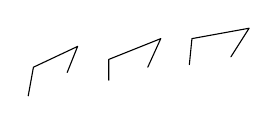
\begin{tikzpicture}[x=0.033cm,y=-0.033cm,line cap=round,line join=round]
\draw (1,19)--(3,8)--(20,0)--(16,10);
\draw (32,13)--(32,5)--(52,-3)--(47,8);
\draw (63,7)--(64,-3)--(86,-7)--(79,4);


\end{tikzpicture}}

$c'_{\beta\gamma}\,(\beta\leq\gamma$

\figure{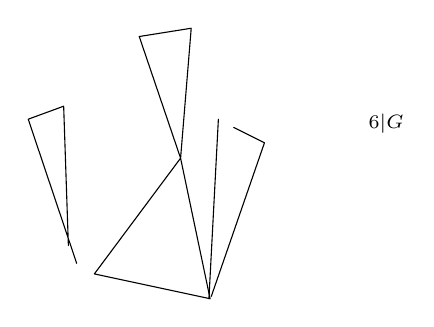
\begin{tikzpicture}[x=0.015cm,y=-0.015cm,line cap=round,line join=round]
\draw (109,1711)--(182,1613)--(207,1732)--cycle;
\draw (182,1613)--(147,1510)--(191,1503)--cycle;
\draw (206,1732)--(214,1580);
\draw (227,1587)--(253,1600)--(208,1730);
\draw (94,1702)--(53,1580)--(83,1569)--(87,1687);

\node[inner sep=1pt,font=\scriptsize] at (356,1584) {$\unsure{6|G}$};
\end{tikzpicture}}

\[
\begin{aligned}
c'_{-1,\gamma}&=6(1+c_\gamma)(1+2c_\gamma)\\
&6.\left|\begin{array}{l}1.1\\2.3\\3.5\\5.9\end{array}\right.
\end{aligned}
\]

\diagram{\(\begin{array}{c|c|c|c|c|}
{}_{\beta}\!\backslash^{\gamma}&-1&0&1&2\\\hline
-1&6=2\unsure{\cdot}3&36=2^2.3^2&90=2.3^2.5&270=2.3^3.5\\\hline
0&0&2^3.3^2\unsure{.}&2^4.3^2.5&2^6.3^3.5\\\hline
1&0&0&\begin{gathered}2^4.3^2.5\\=6!=720\end{gathered}&2^6.3^4.5\\\hline
2&0&0&0&2^7.3^{4}.5\\\hline
\end{array}\)}

% archive sheet number: 118
\scanpage{120}
\[
\begin{aligned}
 c'_{-1,\gamma}&=6(1+c_\gamma)(1+2c_\gamma) &&\gamma\geq-1\\
 c'_{0,\gamma}&=c'_{-1,\gamma}\,{\unsure{\nu|V}}_{-1,0,\gamma}=12c_\gamma^2(1+c_\gamma)(1+2c_\gamma) &&\gamma\geq0\\
 c'_{1,\gamma}&=c'_{0,\gamma}\nu_{0,1,\gamma}=12c_\gamma^2(c_\gamma+1)(c_\gamma-1)(2c_\gamma+1) &&\gamma\geq\deleted{\unsure{0}}\unsure{1|0}\\
 c'_{2,\gamma}&=c'_{1\gamma}\nu_{1,2,\gamma}=12c_\gamma^{\unsure{2|1}}(c_\gamma+1)(c_\gamma-1)(\deleted{\unsure{2}}c_\gamma\unsure{-|+}2)(2c_\gamma+1) &&\gamma\geq2\text{ i.e. }\gamma=2
\end{aligned}
\]

\[
\begin{aligned}
 c_{-1,\gamma}&=\deleted{\unsure{6+2c_\gamma}\,\unsure{\tfrac16}}\inserted{\tfrac16c'_{-1,\gamma}}(1+c_\gamma)(1+2c_\gamma)\\
 c_{0,\gamma}&=\tfrac1{72}c_{0,\gamma}=\tfrac16c_\gamma^2(c_\gamma+1)(c_\gamma-1)(2c_\gamma+1)\\
 c_{1,\gamma}&=\tfrac1{720}c'_{1,\gamma}=\tfrac1{60}c_\gamma^2(c_\gamma-1)(c_\gamma+1)(2c_\gamma+1)\\
 c_{2,\gamma}&=1\quad\text{---}
\end{aligned}
\]

\diagram{\(\begin{array}{c|c|c|c|c|}
 {}_\beta\!\backslash^{\gamma}&-1&0&1&2\\ \hline
 -1&1&6=2\cdot3&15=3\cdot5&45=3^2\cdot5\\ \hline
 0&0&1&10=2\cdot5&\deleted{\unsure{40|12}}120=2^3\cdot3\cdot5\\ \hline
 1&0&0&1&36=2^2\cdot3^2\\ \hline
 2&0&0&0&1\\ \hline
\end{array}\)}

% archive sheet number: 119
